\section{Raccomandazioni o Linee Guida}

La funzione della ricerca scientifica e in particolare della ricerca epidemiologica è il beneficio del paziente e il beneficio della comunità (sanità pubblica).

Sono già state trattate a lezione la ricerca scientifica, i disegni di studio, la letteratura primaria e secondaria, le revisione sistematica e metanalisi.

Manca il concetto delle \textbf{\emph{RACCOMANDAZIONI}}.

I ricercatori fanno ricerca, pubblicano il risultato di tali ricerche nelle revisioni sistematiche e tutto questo serve per sviluppare delle \emph{RACCOMANDAZIONI O LINEE GUIDA}. Le linee guida o protocolli vengono stilate da panels di esperti che si basano sulle \textbf{evidenze} della letteratura.

\begin{figure}[!ht]
\centering
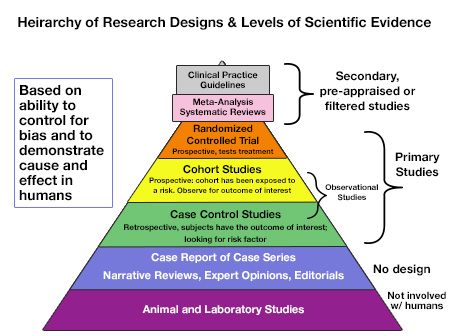
\includegraphics[width=0.7\textwidth]{05/image1.png}
\end{figure}

La \textbf{\emph{piramide delle evidenze}} mostra i vari metodi di studio e di indagine e li va a suddividere a seconda della loro importanza. All'apice della piramide abbiamo le linee guida sulla clinical practice, poi metanalisi e revisioni sistematiche, studi clinici randomizzati e così via.

L'OMS si occupa di stilare le linee guida (che valgono a livello nazionale) attinenti ai vari argomenti clinici e verranno poi implementate a livello degli stati membri.

Arrivare ad una linea guida è un processo molto lungo e che richiede l'azione di più esperti.

\subsection{Medicina basata sulle Evidenze}

La MEDICINA BASATA SULLE EVIDENZE è l'integrazione della migliore ricerca scientifica, con l'aggiunta dell'esperienza clinica del medico e i valori del paziente. (Sackett)

\begin{figure}[!ht]
\centering
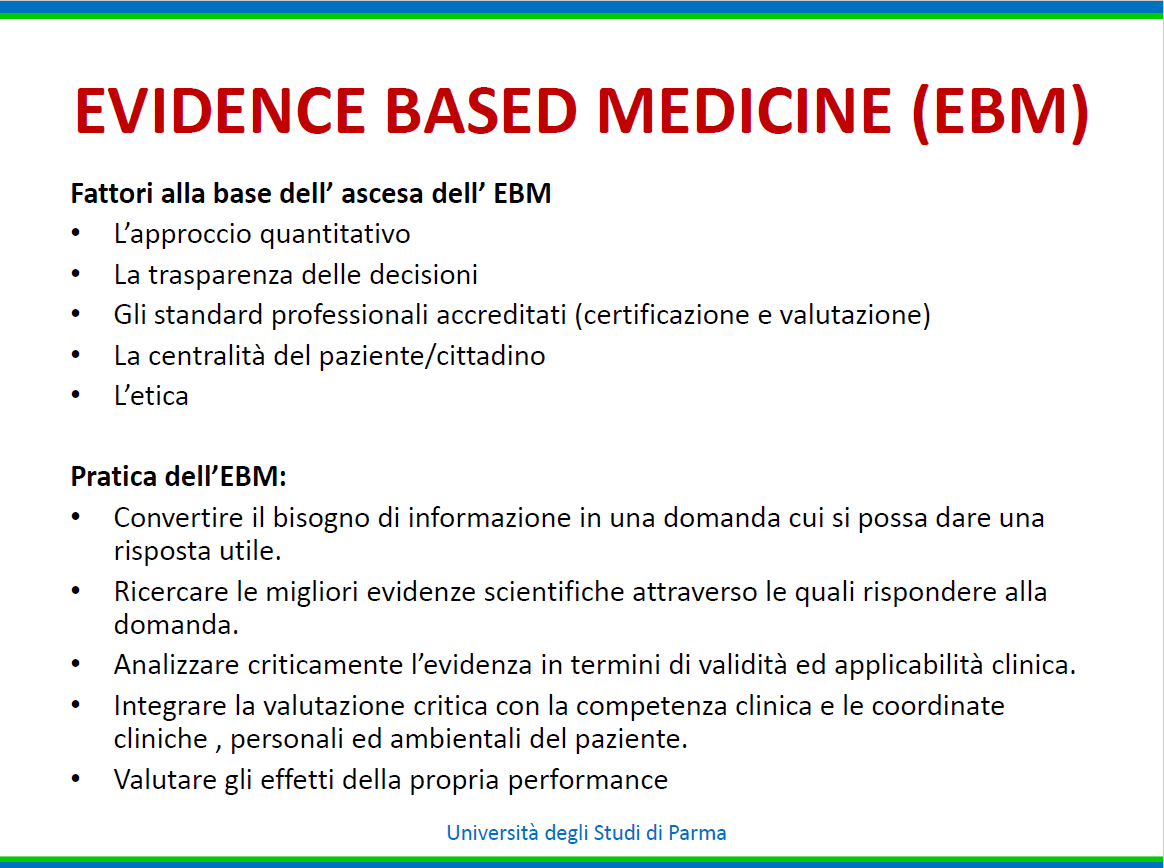
\includegraphics[width=0.7\textwidth]{05/image2.png}
\end{figure}

Tenendo in considerazione ciò che ha detto Sackett, quindi, l'EMB è il risultato di una triangolazione tra:

\begin{itemize}
\item
  applicazione delle evidenze delle ricerche scientifiche
\item
  esperienza clinica da parte del medico
\item
  bisogni clinici e sociali dei pazienti
\end{itemize}

La EMB nasce dalla necessità di sostenere le attività cliniche attraverso principi condivisi di interpretazione dei risultati della ricerca clinica. E' l'uso coscienzioso, esplicito e giudizioso della miglior attuale evidenza scientifica, per prendere decisioni, in relazione all'assistenza sanitaria dei pazienti.

La ricerca scientifica serve ad avere una buona clinica. Qualunque branca della medicina agisce grazie alle evidenze che vengono pubblicate sulle ricerche scientifiche.

\begin{figure}[!ht]
\centering
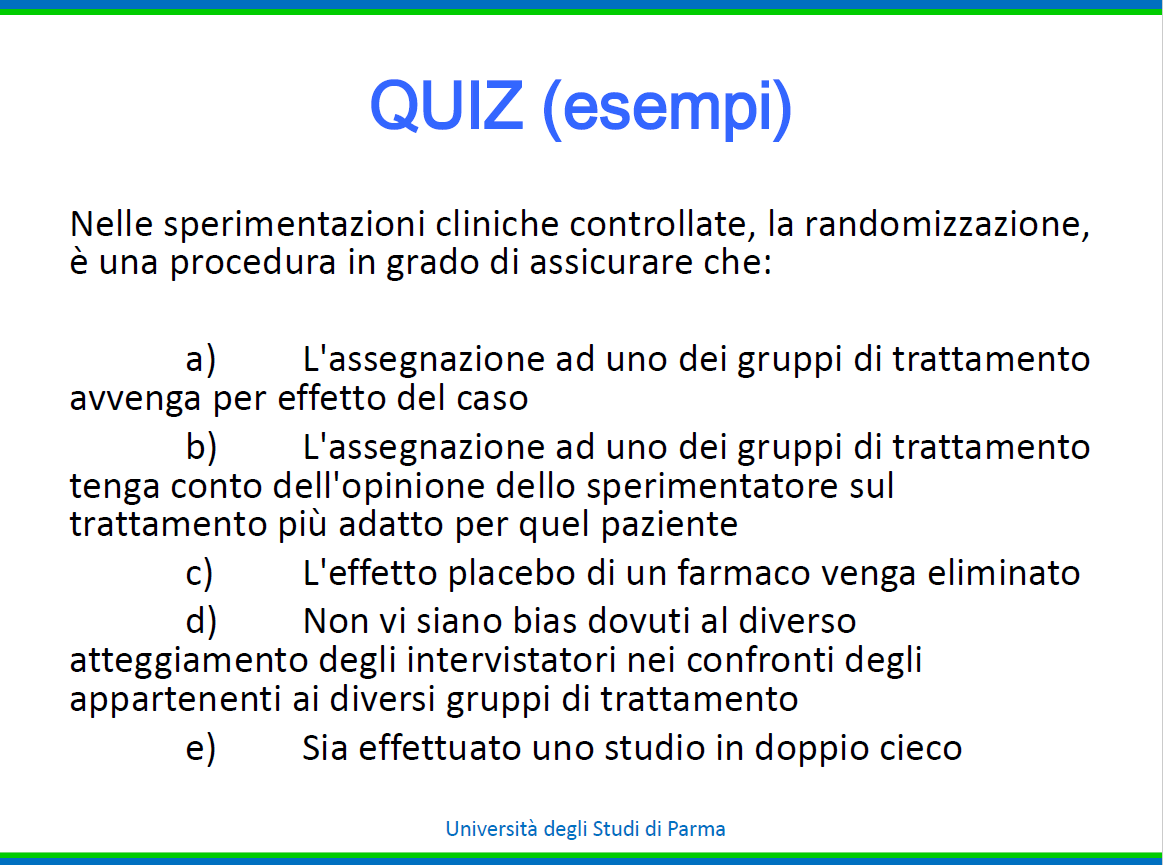
\includegraphics[width=0.7\textwidth]{05/image3.png}
\end{figure}

La risposta corretta è la A.

\begin{figure}[!ht]
\centering
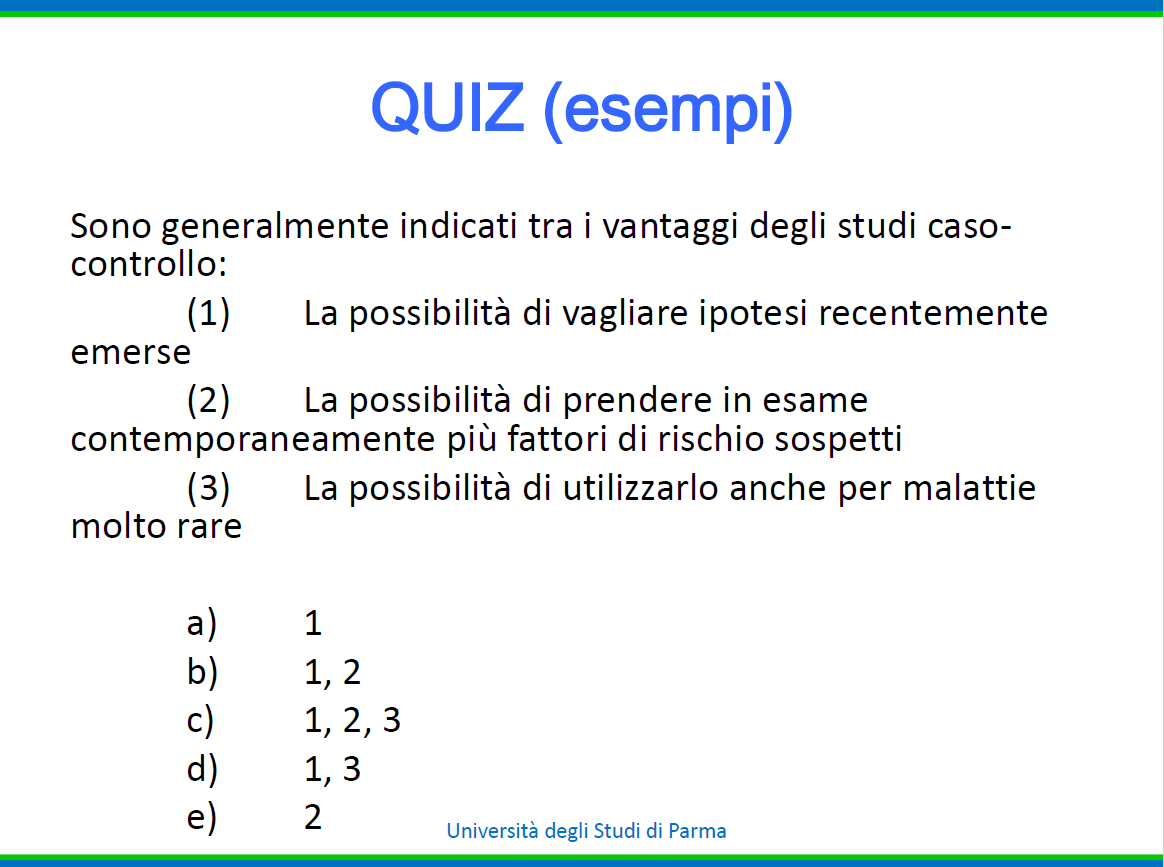
\includegraphics[width=0.7\textwidth]{05/image4.png}
\end{figure}

La risposta corretta è la C.

Lo studio caso-controllo è quello che prende i malati e i non malati e \emph{valuta l'ESPOSIZIONE}. Con questo approccio possiamo \textbf{\emph{indagare più fattori di rischio}} sui malati, mentre \emph{se partiamo dai fattori di rischio} degli esposti e non esposti, sarà \emph{più difficile prendere in considerazione più esposizioni.}

\begin{figure}[!ht]
\centering
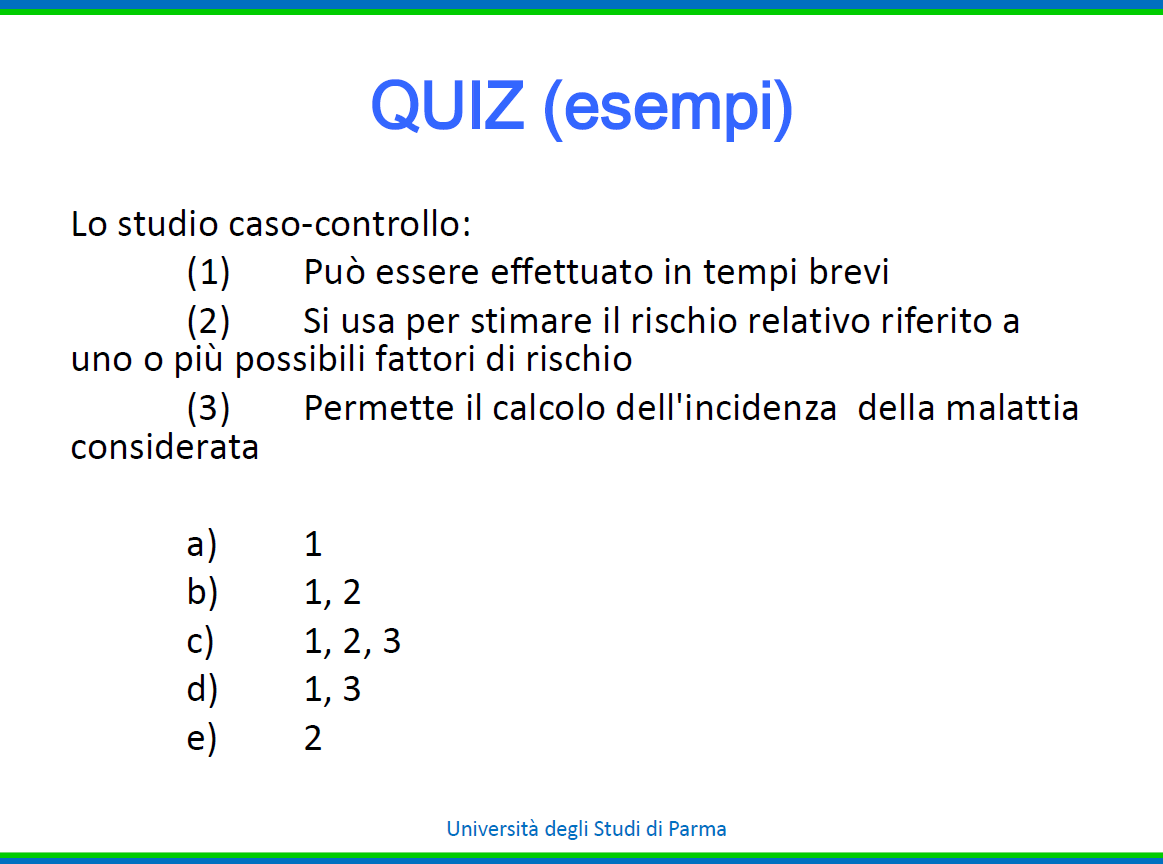
\includegraphics[width=0.7\textwidth]{05/image5.png}
\end{figure}

La risposta corretta è la B.

Lo studio caso-controllo \textbf{\emph{non permette assolutamente il calcolo dell'incidenza della malattia}} considerata. Si calcola in tempi brevi, diversamente da quello che succede con gli studi prospettici.

Non si calcola il rischio relativo degli studi caso-controllo, bensì l'\textbf{\emph{ODDS RATIO}} (che è una stima del rischio relativo, che si avvicina al rischio relativo tanto più la patologia è rara).

\section{Errori in epidemiologia: BIAS e CONFONDIMENTO}

L'obiettivo degli studi epidemiologici di tipo analitico è quello di \textbf{\emph{stimare l'associazione tra un'esposizione e un outcome}}, cioè \textbf{\emph{determinare l'associazione di un fattore di rischio,}} determinante una causa e una patologia di interesse. Gli studi epidemiologici però possono avere degli errori, che possono far si che la stima che si va a calcolare sia errata. Quando si può instaurare l'errore? Può instaurarsi in ciascuno dei passaggi attinenti agli studi epidemiologici, ossia: disegno di studio, raccolta dei dati, analisi e interpretazione dei dati.

\begin{figure}[!ht]
\centering
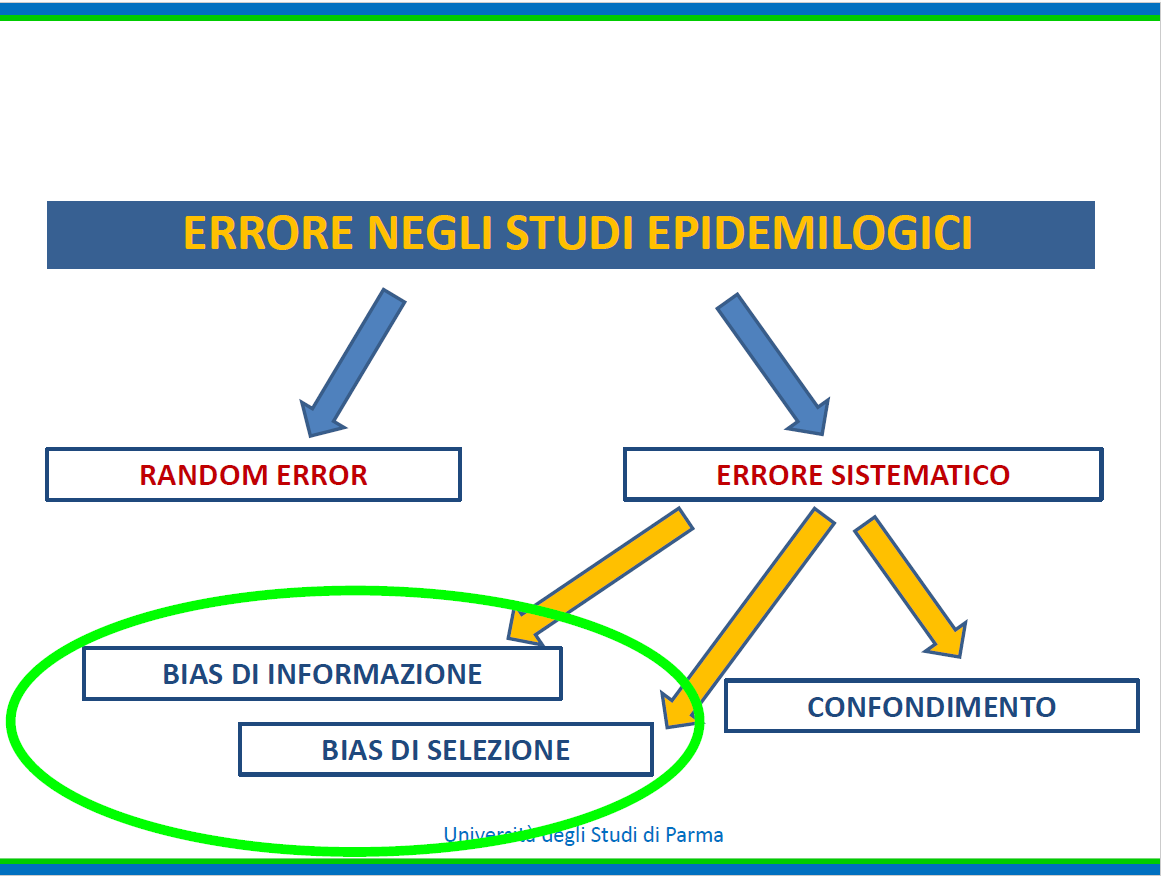
\includegraphics[width=0.7\textwidth]{05/image6.png}
\end{figure}

Tutti gli studi epidemiologici sono potenzialmente a rischio di errore.

Che tipi di errori ci sono? \textbf{\emph{ERRORE RANDOM e ERRORE SISTEMATICO}}

\subsection{Errore Sistematico}

Esso è costituito da due diverse categorie: \textbf{\emph{BIAS e CONFONDIMENTO. }}

Il BIAS è una deviazione dei risultati dal vero; è qualsiasi trend nella raccolta, interpretazione, analisi e review dei dati, che può portare a conclusioni sistematicamente differenti dalla realtà.

Quindi:

\begin{itemize}
\item
  il bias è una forma di distorsione introdotta nei risultati
\item
  i bias possono essere prevenuti attraverso un adeguato disegno sperimentale e una corretta esecuzione dello studio
\item
  i bias non si possono evitare attraverso l'ampliamento della casistica (non dipendono dal numero del campione).
\end{itemize}

I bias sono errori che si instaurano nelle fasi di disegno di studio e nella raccolta dei dati.

Non si può fare molto per minimizzare i bias a livello di analisi dei dati (una volta che i dati sono stati raccolti). Questo è il motivo per cui è necessario spendere adeguate risorse per evitare i bias durante la fase di pianificazione dello studio. I BIAS si suddividono a loro volta in varie categorie:

\paragraph{Bias di Selezione}

Fa riferimento a come gli individui vengono selezionati per prendere parte ad uno studio:

Gli individui selezionati sono rappresentativi della popolazione che si vuole studiare?

\begin{itemize}
\item
  \textbf{\emph{negli studi CASO-CONTROLLO:}} il problema più importante è la selezione dei controlli. Esempi? L'esposizione che si vuole studiare è associata alla probabilità di essere selezionata come controllo. In questo caso i controlli NON sono rappresentativi della popolazione che si vuole studiare.
\end{itemize}

Il bias di selezione fa riferimento ad un \emph{errore} non nella selezione dei casi che vengono selezionati in base all'outcome, bensì \emph{nella selezione dei controlli}.

La selezione dei controlli è in qualche modo associata all'esposizione che si vuole studiare. Ad esempio, vogliamo studiare l'associazione tra fumatori e malati di tumore al polmone. La ricerca dei casi non è difficile: basta prendere i malati di tumore al polmone, dopodichè bisogna valutare una popolazione di controllo sulla quale andare a valutare l'esposizione al fumo per calcolare l'odds ratio quale stima del rischio relativo (odds ratio: valutazione dell'esposizione nei casi e valutazione di esposizione nei controlli, poi si fa il rapporto e tale rapporto rappresenta l'odds ratio, che è uguale, a livello interpretativo, al rischio relativo. Se il risultato è > 1 diciamo che l'esposizione di interesse è un fattore di rischio, se invece il rischio relativo risulta < di 1, l'esposizione di
interesse sarà un fattore protettivo).

Possiamo prendere 100 controlli in via Farini, ad esempio, o 100 controlli in un reparto di ospedale (non in un reparto di oncologia, bensì in un qualsiasi altro reparto). Con questi due tipi di controlli si va a calcolare il rischio relativo. Il calcolo dell'odds ratio come sarà? Si avrà un rischio di neoplasia maggiore nei controlli ospedalieri: è possibile infatti, che i controlli selezionati in ospedale siano più malati rispetto a quelli di via Farini. Il modo in
cui noi andiamo a selezionare i controlli influisce sull'odds ratio!

Ripetendo: non abbiamo nessun problema a selezionare i casi, in questo caso (malati di tumore oppure non malati). La selezione dei controlli (persone sane) è invece difficoltosa! Dobbiamo \textbf{\emph{prendere la popolazione più generale possibile}}, che sia cioè \textbf{\emph{il più
lontano possibile dall'essere un caso}}.

Di solito negli studi caso-controllo, i controlli vengono scelti in ambito ospedaliero, perchè è più semplice, rapido e meno dispendioso in termini economici, ma questo introduce un BIAS DI SELEZIONE. Se invece i
controlli venissero selezionati in modo random nella popolazione
generale, questo si avvicinerebbe di più ad uno studio di tipo
sperimentale. I controlli presi in ambito ospedaliero, infatti,
inficiano la stima relativa dell'odds ratio, perchè sono persone
caratteristicamente diverse dalla popolazione generale, solitamente con
più patologie e morbilità associate. Il fatto di essere in ospedale può
anche condizionare determinate caratteristiche dei pazienti.

\begin{itemize}
\item
  \textbf{\emph{negli studi A COORTE:}} è minore in quanto l'inclusione
  di esposti e non esposti precede l'insorgenza nell'outcome. \emph{Si
  selezionano i pazienti in base all'esposizione (esposti e non esposti)
  e si studia l'insorgenza dell'outcome. }
\end{itemize}

Nel trials, che è la situazione sperimentale per eccellenza, il rischio
di bias è minimo, tranne nei casi in cui ci sia una perdita di follow up
maggiore tra le persone sottoposte all'intervento e le persone presenti
nel gruppo di controllo.

\paragraph{Bias di Informazione}

Fa riferimento alla \textbf{\emph{MISCLASSIFICAZIONE tra esposizione/non
esposizione e/o outcome/non outcome.}} Si deve considerare il fatto che,
in questo tipo di studi, i soggetti malati hanno la tendenza a ricordare
l'esposizione maggiore rispetto ai non malati. Quindi risulta una non
veritiera maggiore esposizione che porta ad una \textbf{\emph{sovrastima
del rischio relativo}}.

\begin{figure}[!ht]
\centering
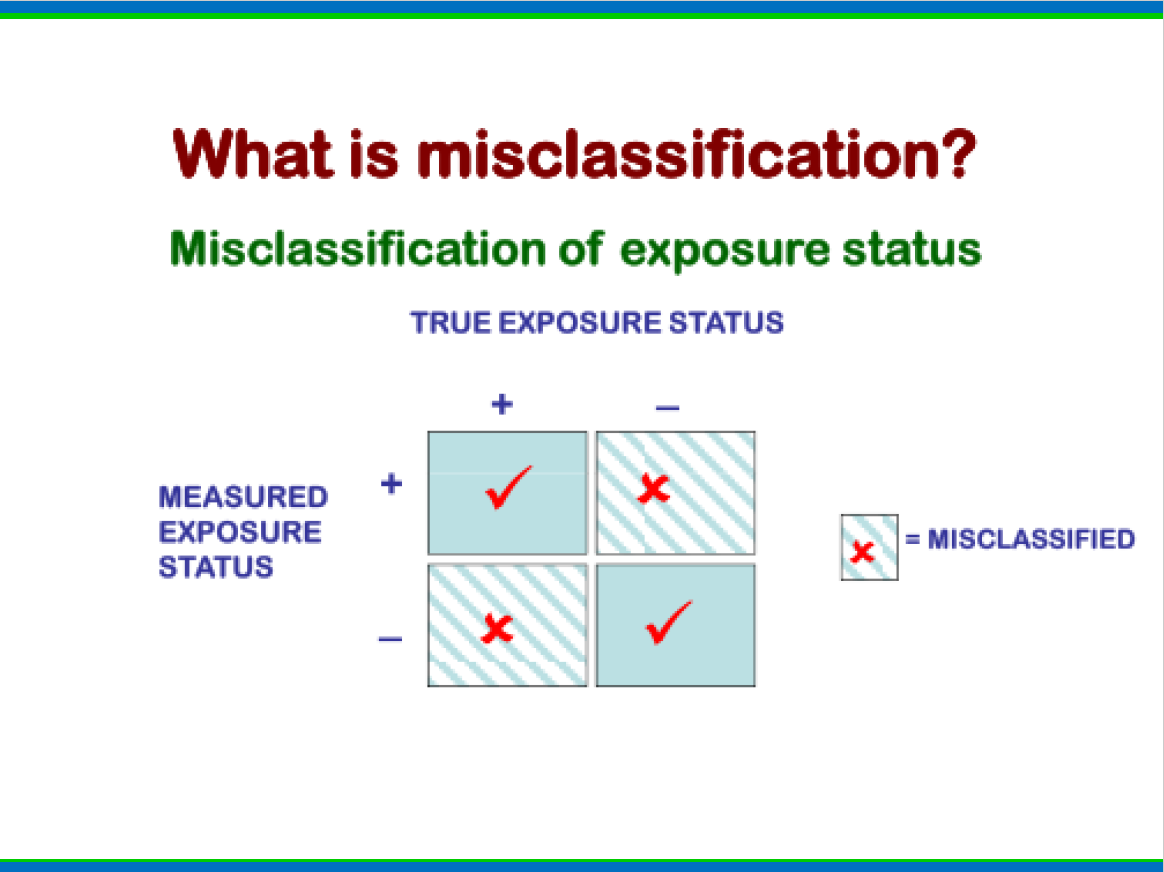
\includegraphics[width=0.7\textwidth]{05/image7.png}
\end{figure}

Guardando l'immagine, lungo la colonna si vede la \emph{vera
esposizione}. Ad esempio: fumatori sì, fumatori no.

Lungo le righe: \emph{esposizione riportata}. Esempio: dicono di essere
fumatori, non dicono di essere fumatori (è difficile non ricordarsi se
si è fumatori oppure no, ma questo è solo un esempio per far capire).

Se l'incrocio tra righe e colonne porta ad un risultato diverso, si
tratta di MISCLASSIFICAZIONE.

Vera esposizione, riportare l'esposizione in maniera corretta; vera non
esposizione, riportare la non esposizione in maniera corretta: queste
sono delle classificazioni corrette. Non lo sono se ad esempio
l'esposizione non c'è ma viene erroneamente riportata.

Questo non si fa per gli studi a coorte perchè, in quel caso, al tempo
0, non c'è nessun malato (persone tutte sane che vanno divise per
diversa esposizione).

Il bias di informazione è perciò un erroneo riportare l'esposizione.
Esso può essere:

\begin{itemize}
\item
  \textbf{\emph{CASUALE}}
\item
  \textbf{\emph{NON CASUALE}}
\end{itemize}

Se è casuale (indipendente dall'outcome o indipendente
dall'esposizione), è semplicemente un errore di misurazione.

Se invece l'errore non è random e se è influenzato dall'outcome e
dall'esposizione, si dice \textbf{\emph{DIFFERENZIALE.}}

Es: stiamo studiando un farmaco che si pensa riesca a curare macchie
cutanee. Vengono presi due gruppi per lo studio: gruppo di malati (con
le macchie cutanee) a cui diamo il farmaco e gruppo di malati a cui non
lo diamo. Dopo un po' di giorni andiamo a vedere l'outcome. Si vede che
le macchie sono diminuite nei pazienti che hanno preso il farmaco. Si
valuta il rapporto della diminuzione delle macchie nei pazienti che
hanno preso il farmaco e il rapporto della diminuzione nei pazienti che
non hanno preso il farmaco. In questo modo si vede l'efficacia del
farmaco.

A volte però l'outcome di interesse non è così oggettivabile: ad esempio
nel caso dei trattamenti con farmaci antidepressivi. Ad un gruppo di
depressi si somministra il farmaco, all'altro gruppo si somministra il
placebo. In questo caso, se io so quale sia il gruppo a cui è stato
somministrato il placebo e quale a cui sia stato somministrato il
farmaco, in una situazione non oggettivabile come questa (lo stato
d'animo dei pazienti), ne potrei essere influenzato e potrei alterare lo
studio.

\emph{\textbf{Bias di informazione di tipo differenziale}: tendo a
considerare come più guarito il paziente che è stato sottoposto al
trattameno. Questo porta ad una sovrastima dell'effetto del farmaco}.

Se invece fossi ignaro riguardo alla suddivisione dei due gruppi, questo
non andrebbe a inficiare sulla valutazione.

Gli effetti della misclassificazione possono quindi essere differenziali
o non differenziali. Se \textbf{\emph{non differenziali, cioè random}},
la stima dell'associazione tra esposizione e outcome è ``biased towards
unity'': \textbf{\emph{l'effetto dell'esposizione è cioè sottostimato.}}

Se invece l'effetto della misclassificazione è
\textbf{\emph{differenziale}}, la stima di associazione tra esposizione
e outcome può essere \textbf{\emph{sia sovra che sottostimato}}, in base
alle circostanze.

\begin{figure}[!ht]
\centering
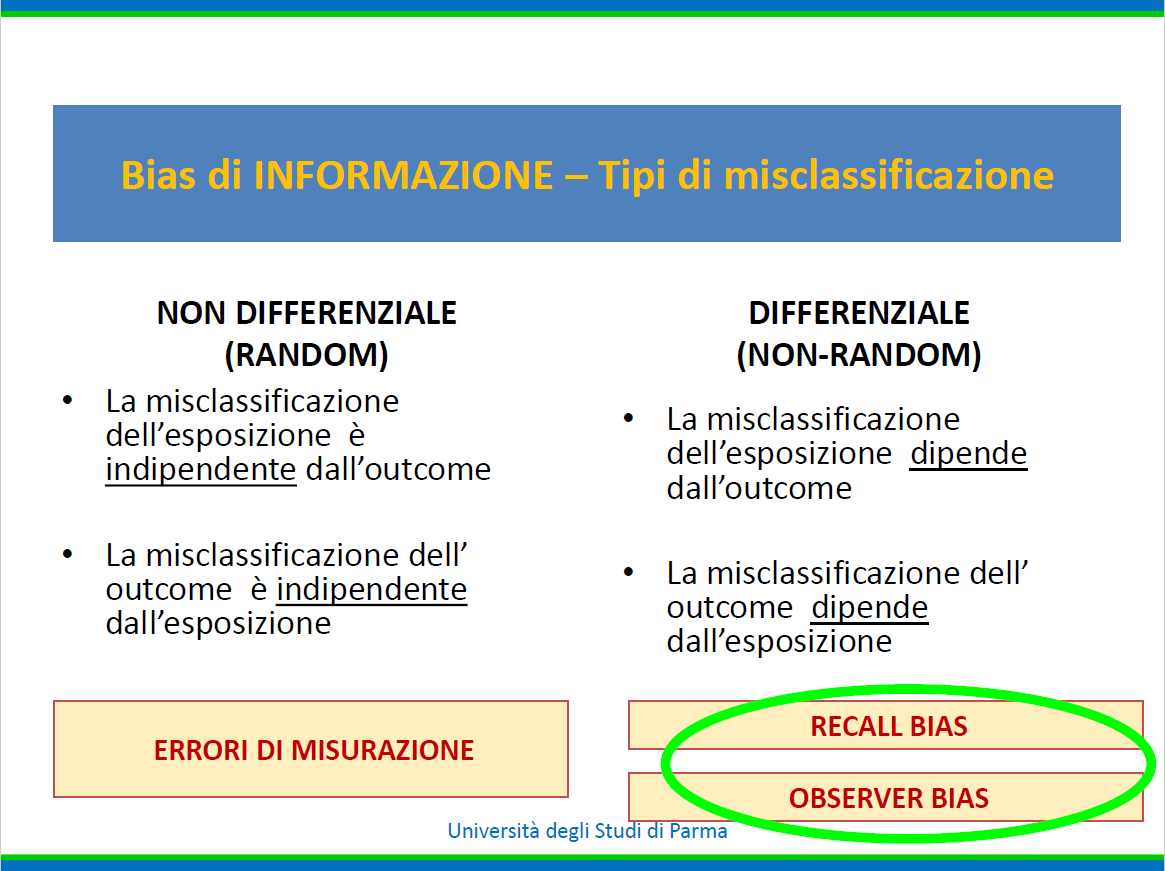
\includegraphics[width=0.7\textwidth]{05/image8.png}
\end{figure}

Il \textbf{RECALL BIAS} è quello del ricordo dell'esposizione; è un
sottotipo di bias di informazione.

E' tipico degli studi caso-controllo; l'accuratezza e l'attendibilità
dell'informazione riportata (e ricordata) dai CASI è superiore a quella
dei CONTROLLI.

COME SI PUO' MINIMIZZARE questo bias?

\begin{itemize}
\item
  facendo interviste standard ai casi ed ai controlli
\item
  usando fonti di dati ogettivi (cartelle cliniche)
\item
  validando il campione delle risposte
\end{itemize}

Ricapitolando: il bias differenziale è in base all'outcome e
all'esposizione. E' un bias che non dipende da errori di misurazione
random, ma è associato al fatto di essere un caso o un controllo: la
misclasificazione è legata allo status di caso, al fatto di essere un
caso o un controllo.

Errore DIFFERENZIALE : la selezione o l'info è sbagliata in maniera
direttamente legata al fatto di essere un caso, un controllo; un
esposto-non esposto.

Errore NON DIFFERENZIALE: l'errore è indifferentemente, in maniera
random, distribuito tra le categorie studiate.

Un esempio classico di information bias, che misclassifica l'esposizione
in base al fatto di essere casi o controlli, è proprio un caso di errore
differenziale, che porta i casi, in maniera differenziale, a
sovrastimare l'esposizione.

Non si tratta di errori di analisi, bensì di errori che avvengono
durante l'attuazione dello studio. L'analisi è un processo in cui non si
verrà più a contatto con i pazienti, ma si studieranno i dati già
ricavati e già opportunatamente trascritti in tabelle excell. Se in fase
di implementazione dello studio sono stati raccolti dei dati sbagliati,
in fase di analisi, ormai, non avrò più la possibilità di minimizzare i
bias.

L' \textbf{OBSERVER BIAS} è un altro tipo di bias d'informazione in cui
l'errore sistematico è dell'osservatore che classifica in base al fatto
che sa a quale gruppi sono stati assegnati i vari soggetti:

\begin{itemize}
\item
  il ricercatore raccoglie dati sull'esposizione in maniera diversa tra
  casi e controlli
\item
  il ricercatore fa diagnosi di outcome in maniera diversa tra
  esposti/non esposti
\end{itemize}

IL RICERCATORE è INFLUENZATO DALL'IPOTESI DI RICERCA.

Come minimizzarlo?

\begin{itemize}
\item
  rendere il ricercatore cieco sullo status di caso/controllo dei
  soggetti (difficile nel caso visto prima, ad esempio, sulle macchie
  cutanee)
\item
  mascherare nei questionari l'ipotesi di ricerca
\item
  utilizzo di misure oggettive e protocolli standard
\item
  training degli operatori
\end{itemize}

\begin{figure}[!ht]
\centering
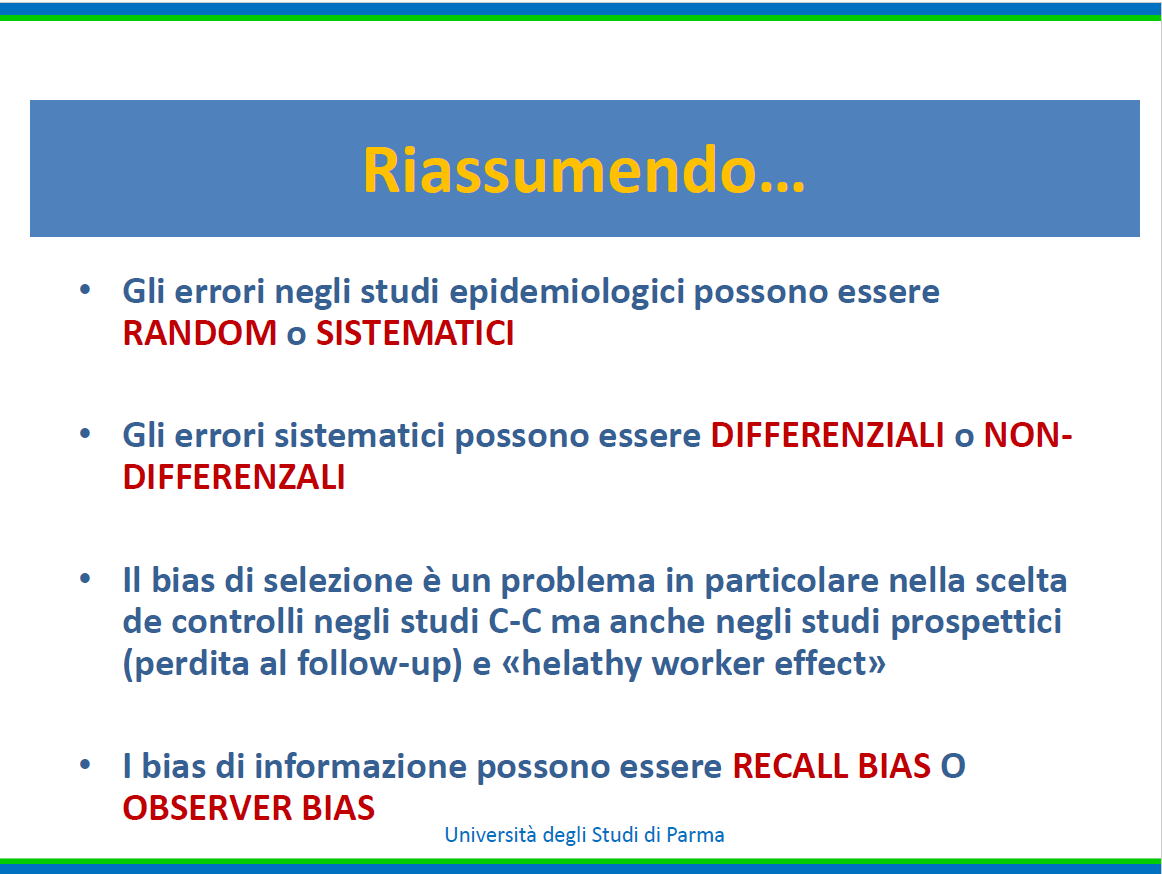
\includegraphics[width=0.7\textwidth]{05/image9.png}
\end{figure}

BIAS DI SELEZIONE, BIAS DI INFORMAZIONE (RECALL BIAS E OBSERVER BIAS,
errore sistematico dell'osservatore che classifica in base al fatto che
sa l'appartenenza dei soggetti ai vari gruppi).

\subsection{Confondimento}

E' un fattore associato sia all'esposizione sia all'outcome.

Se è presente un fattore associato sia all'esposizione che all'outcome e
noi non lo prendiamo in considerazione, sbagliamo.

Es. Vogliamo studiare l'associazione tra colore dei capelli grigi e
presenza di patologia cronica degenerativa. Si prende un gruppo di
persone con i capelli grigi e un gruppo di persone con i capelli di
altri colori e si studia l'insorgenza di patologie cronico-degenerative.
Si scopre che l'incidenza di questo tipo di patologie è proprio più alta
in chi ha i capelli grigi. Quindi, l'avere i capelli grigi è un fattore
di rischio? Assolutamente no! C'è un confondimento, sia legato
all'esposizione, sia all'outcome. Tale confondimento potrebbe essere
l'età. Se tenessi conto dell'età, troverei un rischio relativo attorno
all'uno e che quindi mi indicherebbe che il fatto di avere i capelli
grigi di per sè, non è un fattore di rischio.

Il confondimento può essere eliminato in fase di analisi. Si può
eliminare con delle tecniche statistiche multivariabili che riescono a
valutare il rischio relativo tra capelli grigi e patologia tenendo conto
dell'età, oppure stratificando in vari gruppi di età diverse. Facendo
ciò si va a minimizzare il confondimento.

Non sempre è così facile andare a valutare quale sia il fattore di
confondimento. Ci possono essere molteplici fattori che influenzano i
miei dati, oltre all'età: ad esempio: lo stato socio-economico,
l'istruzione, il peso, varie comorbidità. In fase di analisi, gli studi
migliori sono quelli che tengono in considerazione questi vari possibili
fattori di confondimento e che riescono a denaturare l'analisi,
minimizzandola all'effetto dell'esposizione di interesse e all'outcome.

L'epidemiologia cerca di stimare i determinanti, le varie cause, tenendo
sempre in considerazione tutti i possibili fattori di confondimento.

\subsection{Errore Random}

Noi vogliamo studiare quello che avviene a livello di popolazione, ma
quello che in realtà facciamo è \emph{studiare un piccolo campione di
popolazione} (\textbf{errore campionario}). Per questo motivo, un errore
in questi studi c'è sempre, ed è un errore affidato al caso. In fase di
disegno di studio questo errore non si può eliminare: è INELIMINABILE.
E' stimabile con tecniche statistiche in fase di analisi.

L'errore casuale è tanto più grande quanto più piccolo è il campione.

L'errore sistematico di selezione è un errore che viene fatto in fase di
disegno e conduzione dello studio. Lo si può minimizzare con degli
accorgimenti, in fase di analisi, ma non eliminare del tutto.

\section{Lo sviluppo di un farmaco}

\begin{figure}[!ht]
\centering
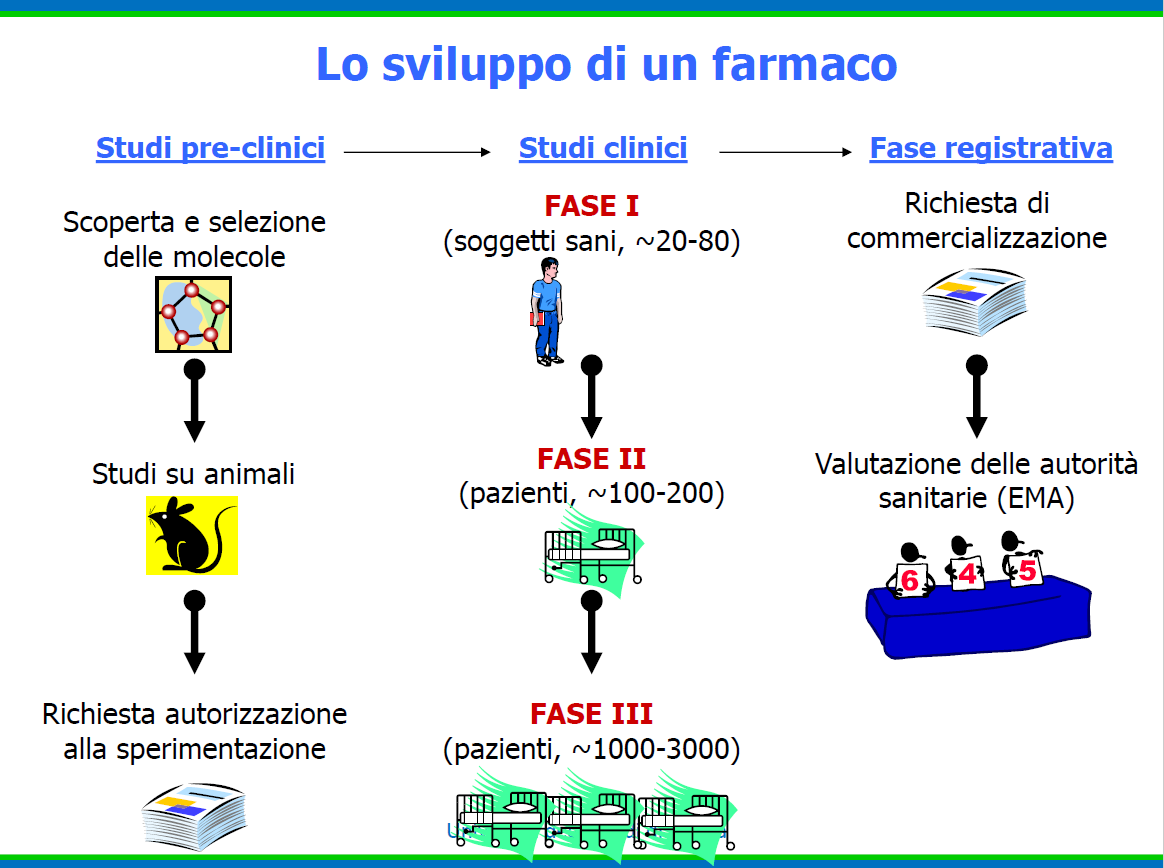
\includegraphics[width=0.7\textwidth]{05/image10.png}
\end{figure}

Le fasi per lo sviluppo di un farmaco sono tre:

\begin{itemize}
\item
  studi clinici
\item
  studi pre-clinici
\item
  fase registrativa
\end{itemize}

Gli studi pre-clinici sono quelli che vengono fatti sugli animali,
terminati i quali sarà possibile richiedere l'autorizzazione per la
sperimentazione, dando così inizio alla fase successiva.

Gli studi clinici si dividono in: fase 1, fase 2, fase 3, tra le quali
varierà il numero di soggetti sottoposti allo studio.

Nella fase di registrazione abbiamo la richiesta di commercializzazione
di un farmaco, che verrà valutata dalle autorità nazionali, tra le
quali, a livello Europeo, abbiamo l'EMA (European Medicine Authority),
mentre in Italia abbiamo l' AIFA (agenzia Italiana del farmaco).

Per alcuni farmaci è richiesta l'autorizzazione a livello Europeo, per
altri, a livello Nazionale.

Gli studi clinici di \textbf{fase 1} hanno una durata di un anno o due,
vengono fatti su soggetti di età compresa tra i 20 e 80 anni, volontari
sani. Vanno a studiare:

\begin{itemize}
\item
  la tollerabilità e sicurezza di un farmaco
\item
  i dati di farmaco-cinetica
\item
  i dosaggi ottimali da impiegare durante la fase 2
\end{itemize}

Anche gli studi di \textbf{fase 2} hanno una durata di 1 o 2 anni.
Vengono svolti su di un numero maggiore di soggetti (centinaia).
Valutano:

\begin{itemize}
\item
  l'efficacia e la tollerabilità del farmaco nei PAZIENTI (cioè in
  soggetti malati)
\item
  l'individuazione del rapporto dose-effetto
\end{itemize}

Gli studi di \textbf{fase 3} sono studi più lunghi (3-4 anni), vengono
fatti su più pazienti (1000-3000), per:

\begin{itemize}
\item
  la valutazione di efficacia e tollerabilità su di un campione AMPIO
\item
  definizione finale tra dose ed effetto
\item
  confronto tra trattamenti diversi
\end{itemize}

Gli studi di \textbf{fase 4} sono quelli di post-marketing e sono i più
lunghi in assoluto: durano per sempre. I soggetti interessati sono tutti
coloro che vengono sottoposti ad un determinato trattamento. Gli
obiettivi sono:

\begin{itemize}
\item
  rilevazione di risposte rare/eventi avversi
\item
  effetto dell'interazione con altri farmaci
\end{itemize}

Quando sono nati i trials clinici? Il primo trial è stato effettuato nel
1948, per il trattamento della tubercolosi, con la STREPTOMICINA. I
soggetti sottoposti allo studio avevano un'età compresa tra i 15 e i 25
anni ed erano randomizzati. Si fece l'analisi dei risultati dopo 6 mesi
di trattamento.

\begin{figure}[!ht]
\centering
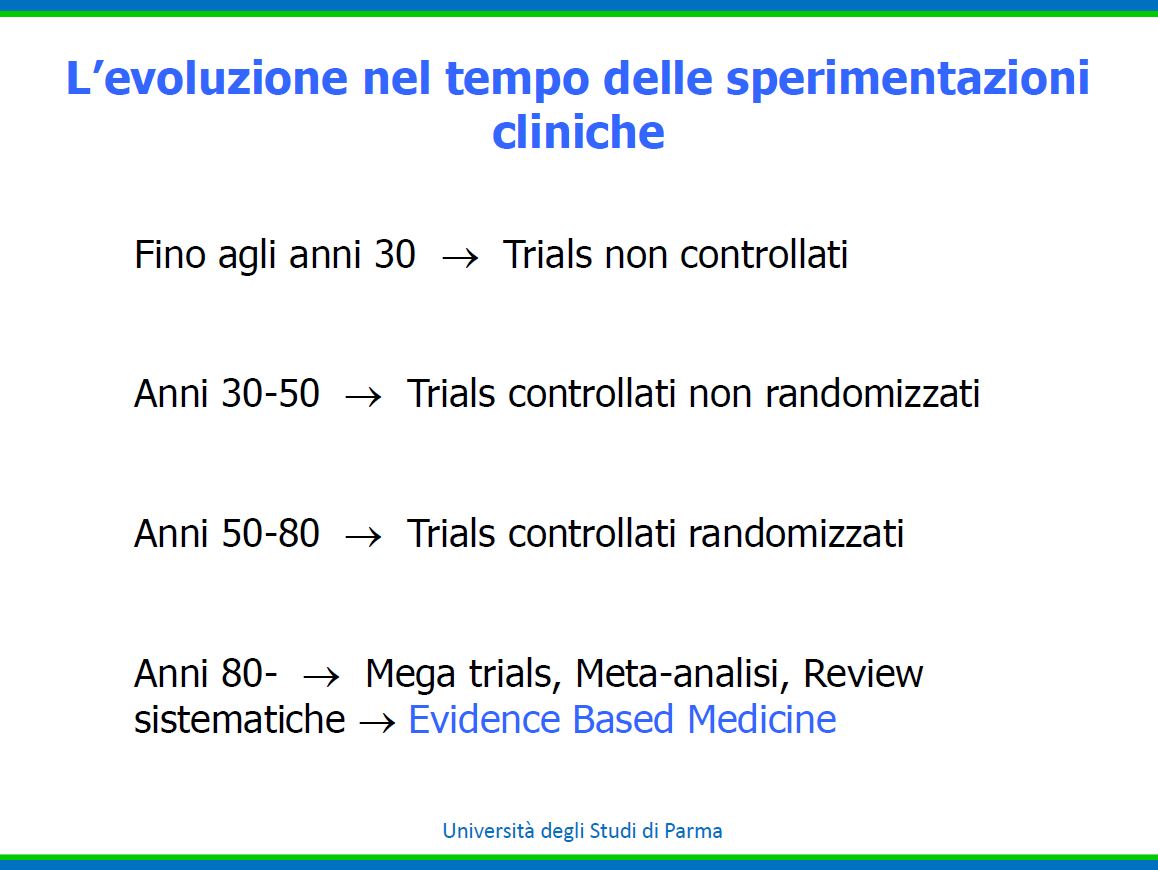
\includegraphics[width=0.7\textwidth]{05/image11.png}
\end{figure}

\subsection{Criteri per una corretta sperimentazione clinica sui farmaci}

\begin{figure}[!ht]
\centering
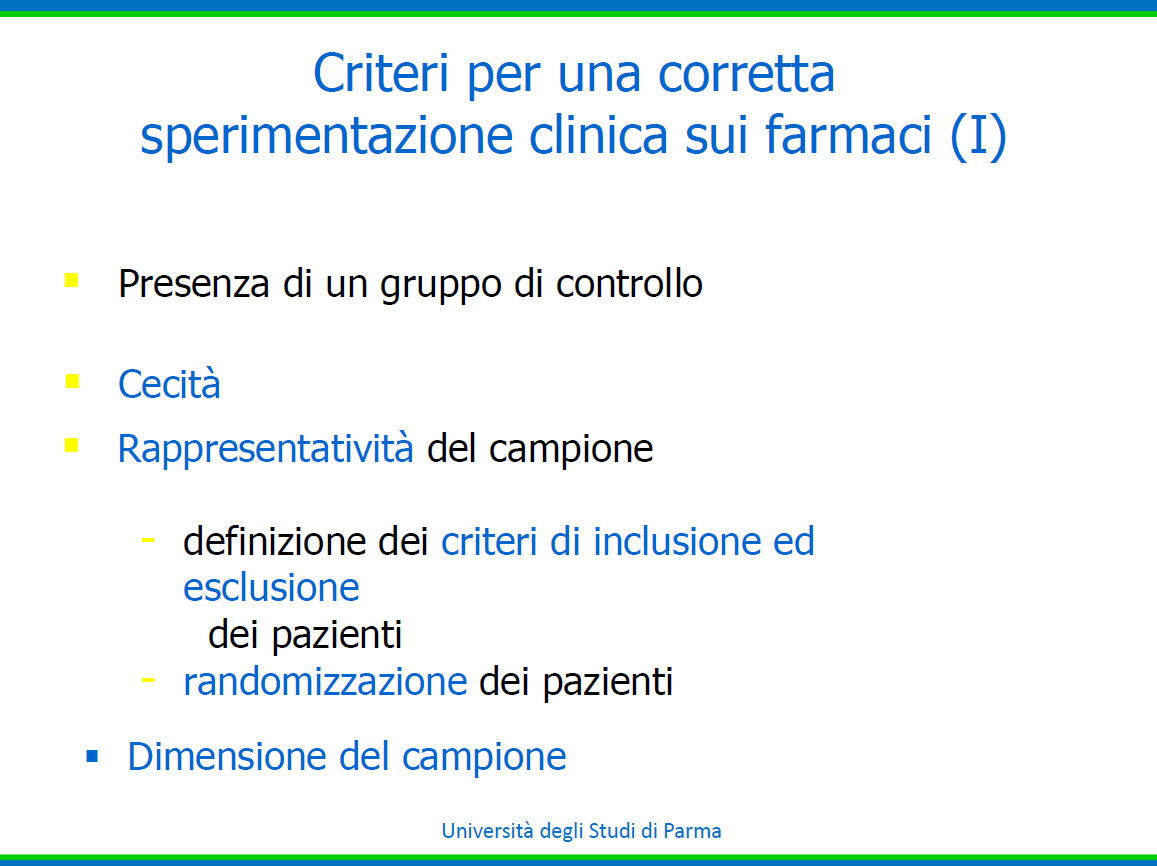
\includegraphics[width=0.7\textwidth]{05/image12.png}
\end{figure}

\textbf{1. Presenza di un gruppo di controllo}

Per gli studi epidemiologici è fondamentale la presenza di un
\textbf{\emph{gruppo di controllo}}. Questi gruppi di controllo possono
essere di tipi diversi:

\textbf{Gruppi paralleli}: gruppo A che fa un trattamento, gruppo B che
assume un altro farmaco o placebo, seguiti nel tempo

\textbf{Disegno cross-over}: ciascun gruppo riceve lo stesso trattamento
in fasi successive del trials. E' questo un disegno di studio più
complicato. I suoi:

\begin{itemize}
\item
  \textbf{vantaggi} sono: minor variabilità, miglior utilizzo del
  campione.
\item
  \textbf{svantaggi}: si può applicare solo in determinati trattamenti
  (soprattutto cronici) e la difficoltà di studio è maggiore rispetto a
  quella dei gruppi paralleli.
\end{itemize}

\begin{figure}[!ht]
\centering
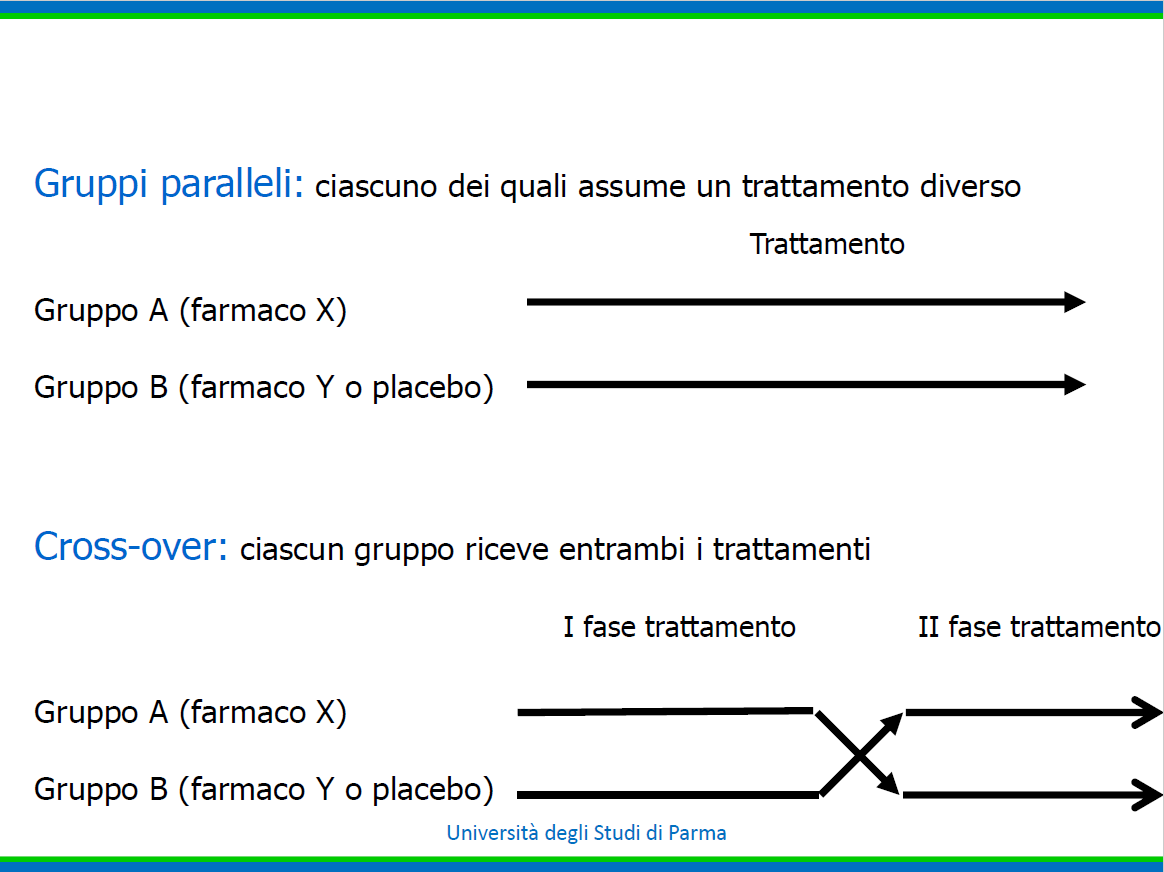
\includegraphics[width=0.7\textwidth]{05/image13.png}
\end{figure}

\textbf{2. BLINDNESS, CECITA'}

Ci può essere a due livelli: a livello del paziente, che non sa a che
gruppo è stato assegnato (\textbf{singolo} \textbf{cieco}) e anche a
livello dello sperimentatore (\textbf{doppio cieco}). Questo impedisce
di essere influenzati dalle aspettative che si hanno da un determinato
trattamento. Altrettanto importante è essere ciechi sulla analisi e
valutazione degli studi.

\textbf{3. RAPPRESENTATIVITA' del campione}

Il campione sul quale noi facciamo ricerca è assimilabile alla
popolazione a cui vogliamo assegnare le conclusioni del nostro studio:

\textbf{3A. CRITERI DI INCLUSIONE ED ESCLUSIONE DEI PAZIENTI}

A partire dalla popolazione generale noi applichiamo dei criteri di
eleggibilità e otteniamo la popolazione oggetto di studio. Reclutiamo
attivamente dei pazienti e abbiamo il campione. Facciamo degli studi sul
campione, ma vogliamo che i risultati dello studio si riferiscano alla
popolazione generale. Questo concetto si definisce
\textbf{\emph{INFERENZA STATISTICA}}. Ossia: \emph{la popolazione è la
collettività di soggetti oggetto di studio. Il campione è invece il
gruppo di soggetti estratti dalla popolazione.}

La casualità del campione permette di utilizzare le procedure
dell'inferenza statistica trasferendo i risultati alla popolazione.

Il problema dei trials è la definizione della popolazione (criteri di
inclusione ed esclusione) e l'estrapolazione dei risultati ad una
popolazione più generale rispetto a quella oggetto di studio.

\textbf{3B. La randomizzazione dei pazienti}

E' una caratteristica fondamentale dei trials clinici. I pazienti,
reclutati sulla base dei criteri di inclusione ed esclusione statistici,
vengono assegnati al gruppo di trattamento o di controllo mediante una
forma più o meno sofisticata di sorteggio o randomizzazione (il pc
genera sequenze numeriche casuali).

La randomizzazione deve rendere imprevedibile a quale trattamento verrà
assegnato il paziente successivo. In questo modo si riescono ad ottenere
dei \emph{gruppi omogenei} tra di loro per tutte le caratteristiche note
ed ignote, \emph{ad esclusione del trattamento}: i due gruppi saranno
omogenei, eccezion fatta per il trattamento testato.

L'omogeneità sarà maggiore in relazione alla numerosità del campione.

Insieme alla randomizzazione viene spesso applicata la
\textbf{\emph{STRATIFICAZIONE DEL CAMPIONE }}

\begin{figure}[!ht]
\centering
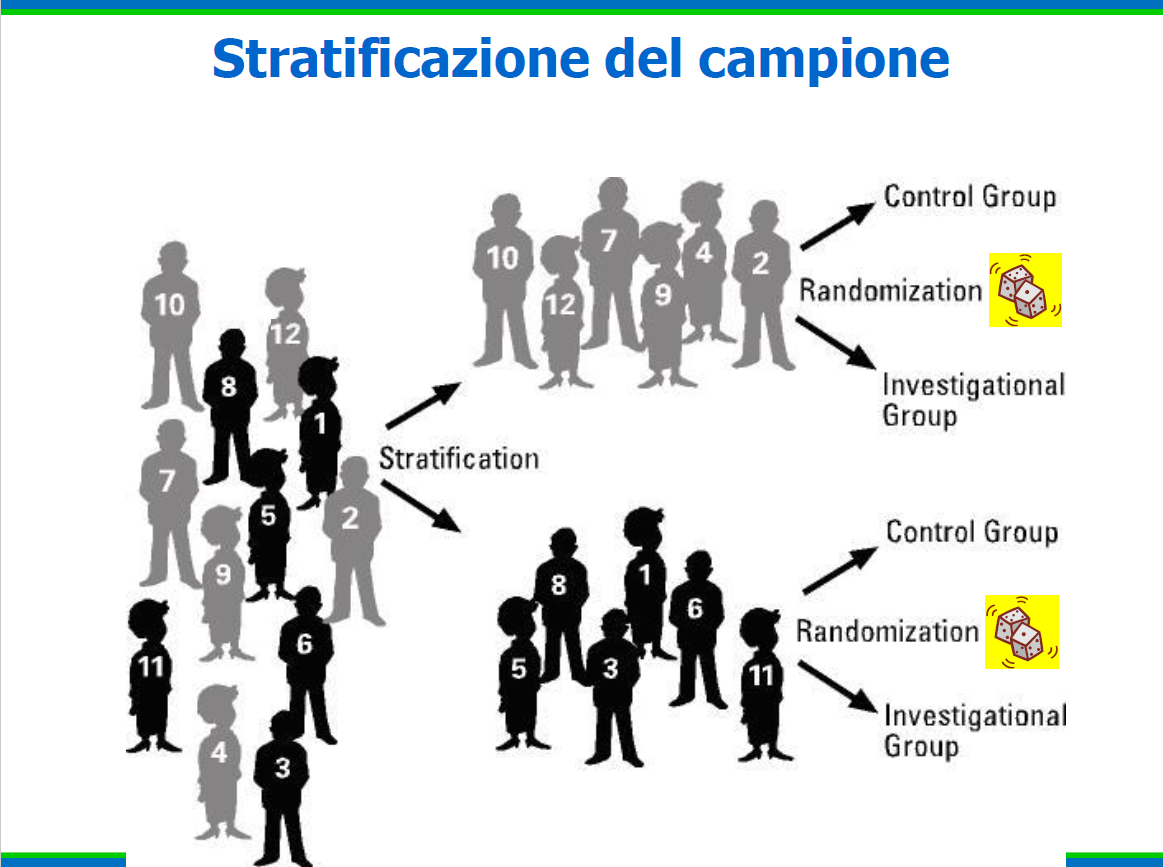
\includegraphics[width=0.7\textwidth]{05/image14.png}
\end{figure}

Se ci interessa sapere se i risultati dello studio sono validi in
maniera stratificata, cioè se il trattamento ha lo stesso effetto, ad
esempio, sui maschi e sulle femmine, prima di randomizzare i pazienti li
stratifichiamo per età, per genere, per sesso (in pratica per la
stratificazione che ci interessa valutare).

I risultati di uno studio sono estrapolabili solo ai soggetti con le
stesse caratteristiche dei reclutati. Se facciamo uno studio riferendoci
ad una particolare etnia, lo studio può essere estrapolabile anche ad
una etnia diversa da quella studiata? No!

E' quindi opportuno scegliere criteri di inclusione non troppo rigidi,
perchè altrimenti non si avrebbe la certezza che i dati ottenuti
potrebbero andare bene anche su altre popolazioni.

Molto spesso vengono esclusi dalla ricerca donne in gravidanza, anziani,
bambini.... che sono comunque pazienti che spesso usano proprio quei
farmaci in corso di studio!

\textbf{4. DIMENSIONE DEL CAMPIONE}

La numerosità del campione deve essere tale da rispondere
all'obiettività dello studio. Non dovrebbero mai essere arruolate più
persone di quelle necessarie. Ci sono degli studi statistici che mi
permettono di calcolare quanto grande dovrebbe essere il mio campione:
\textbf{\emph{CALCOLI SUL POTERE STATISTICO DELLO STUDIO.}}

\subsection{Outcome o End Points}

Ci sono altri criteri per la valutazione della sperimentazione: è
importante la scelta degli \textbf{\emph{outcome (o end points)}} sui
quali noi andiamo a valutare il nostro risultato dello studio (esempio,
l'efficacia di un farmaco). Tali outcome devono essere classificati a
priori, prima dello svolgimento dello studio.

Ci sono degli outcome DIRETTI, cioè direttamente misurabili (come ad
esempio, la mortalità totale, la causa di mortalità, eventi non fatali
come per esempio la causa di una frattura di femore).

Ci sono degli outcome INDIRETTI: esempio, le variazioni dei parametri di
laboratorio.

HARD: di sicura determinazione, per la verifica dei quali l'errore è
minimo (la mortalità per esempio).

SOFT: possono essere influenzati da imprecisioni o soggettività
(miglioramento di un quadro sintomatologico, qualità di vita). Sono più
difficili da oggettivare.

Dobbiamo valutar anche gli \textbf{\emph{ASPETTI ETICI e il CONSENSO
INFORMATO}}.

Validità scientifica e valore vanno di pari passo: "bad science, bad
ethics", anche se "good science not always good ethics".

La validità scientifica non comporta il fatto di venir meno ai concetti
di etica.

\subsection{Megatrials}

\begin{figure}[!ht]
\centering
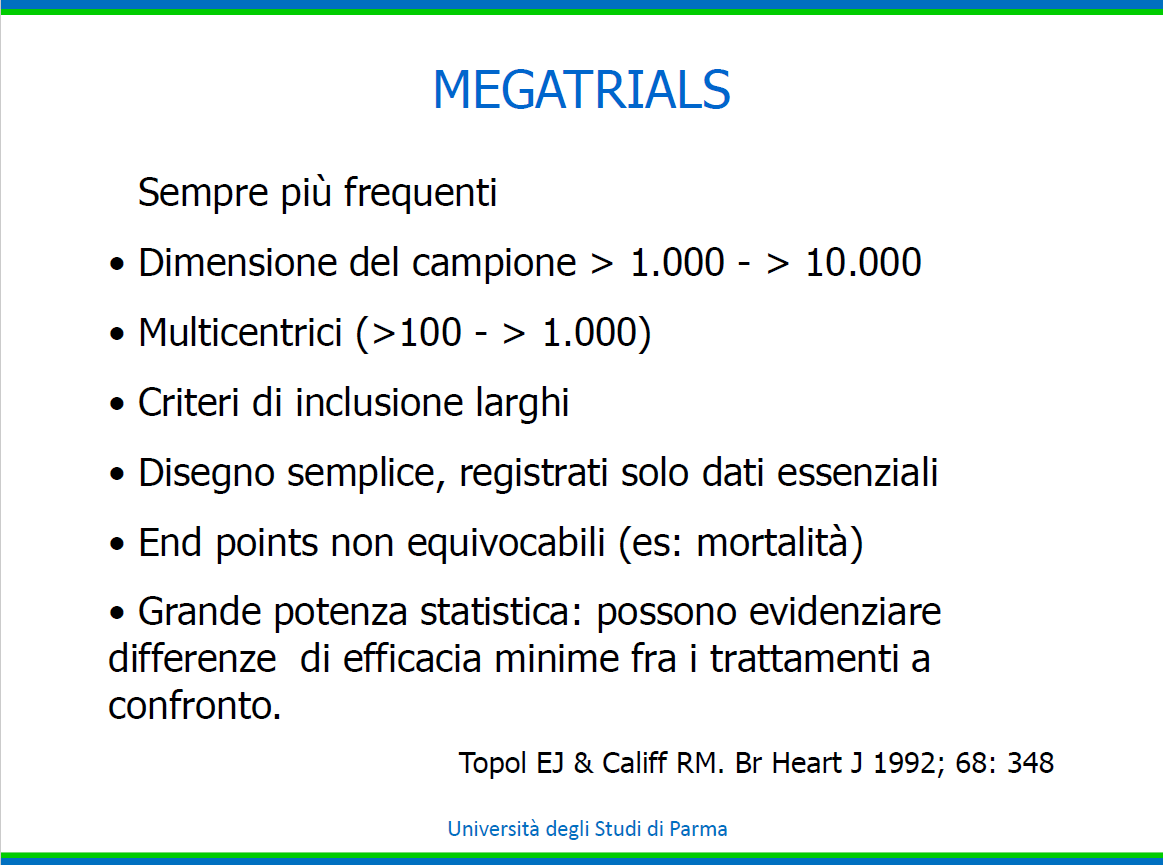
\includegraphics[width=0.7\textwidth]{05/image15.png}
\end{figure}

Si stanno sempre di più facendo i cosiddetti \textbf{\emph{MEGATRIALS}},
al giorno d'oggi. Sono trials che hanno dimensioni del campione molto
più elevate, sono di solito multicentrici, i criteri di inclusione sono
larghi, di disegno semplice e vengono registrati solo i dati essenziali
clinical trials dot com (gli studi clinici vengono registrati in fase di
protocollo, devono essere registrati per legge, e sul protocollo di
registrazione sono indicati i siti, gli ends points, le metodologie con
cui viene fatto lo studio). Gli end points sono non equivocabili e ci
sarà una grande potenza statistica: quanto più sarà grande il campione,
tanto più sarà efficace e preciso lo studio.

\paragraph{MAGNESIO NELL'INFARTO MIOCARDICO: MEGATRIAL}

Per studiare l'efficacia del magnesio su end points di tipo cardiaco
sono stati fatti dei grossi studi clinici randomizzati, dei veri e
propri megatrials.

Razionale: variazione nell'andamento di patologie cardiache in funzione
della quantità di magnesio nell'acqua.

Studi su animali hanno mostrato l'attività antiaritmica, antiaggregante
e coronarodilatatrice del magnesio. Piccoli trials positivi sull'uso del
magnesio nell'infarto. Una review informale dei risultati ha mostrato
una riduzione della mortalità da IMA (infarto miocardico acuto). Una
meta-analisi formale su 1300 pazienti con un totale di 78 decessi ha
mostrato una riduzione del 55\% nel rischio di morte (p= 0,001).

Studio chiamato LIMIT-1 su 100 paz : diminuzione aritmie (1986)

Studio LIMIT-2 su 2300 paz: diminuzione incidenza di insuff.
ventricolare sx (1994)

\begin{figure}[!ht]
\centering
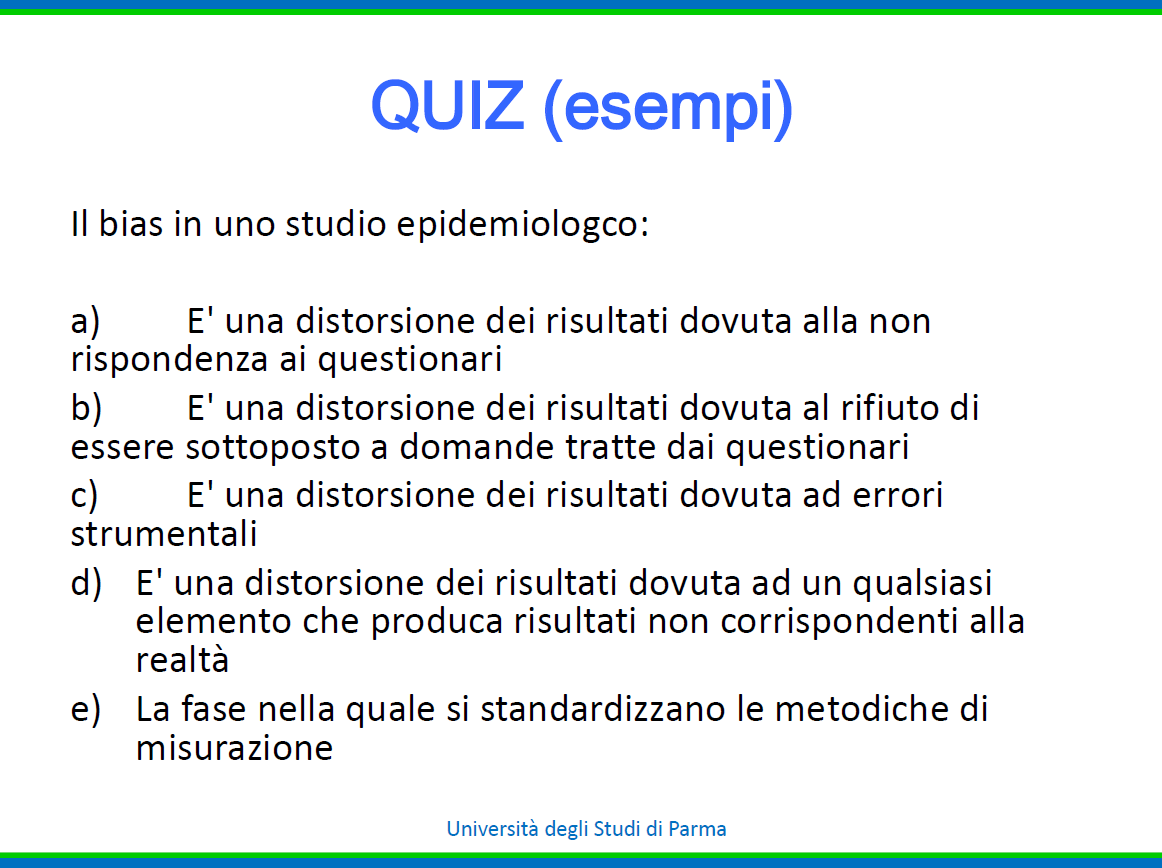
\includegraphics[width=0.5\textwidth]{05/image16.png}
\end{figure}

Risposta: D.

La C è errata perchè errori strumentali non necessariamente determinano
una distorsione dei risultati.

\begin{figure}[!ht]
\centering
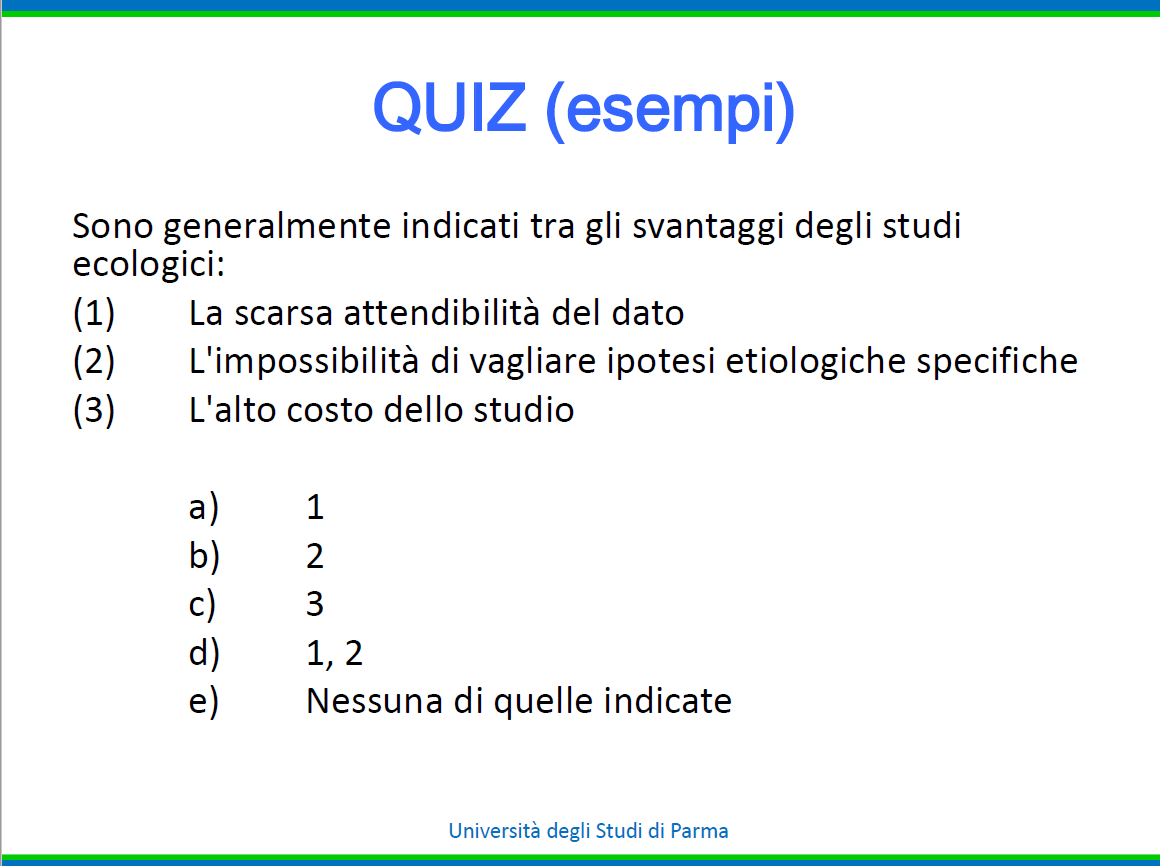
\includegraphics[width=0.5\textwidth]{05/image17.png}
\end{figure}

Risposta: D.
\newpage
Gli studi ecologici danno un dato molto generico, perchè utilizzano dati
amministrativi raccolti in precedenza non a fini di ricerca e quindi
possono riportare dati poco specifici o poco attendibili per il dato che
si sta ricercando.

\begin{figure}[!ht]
\centering
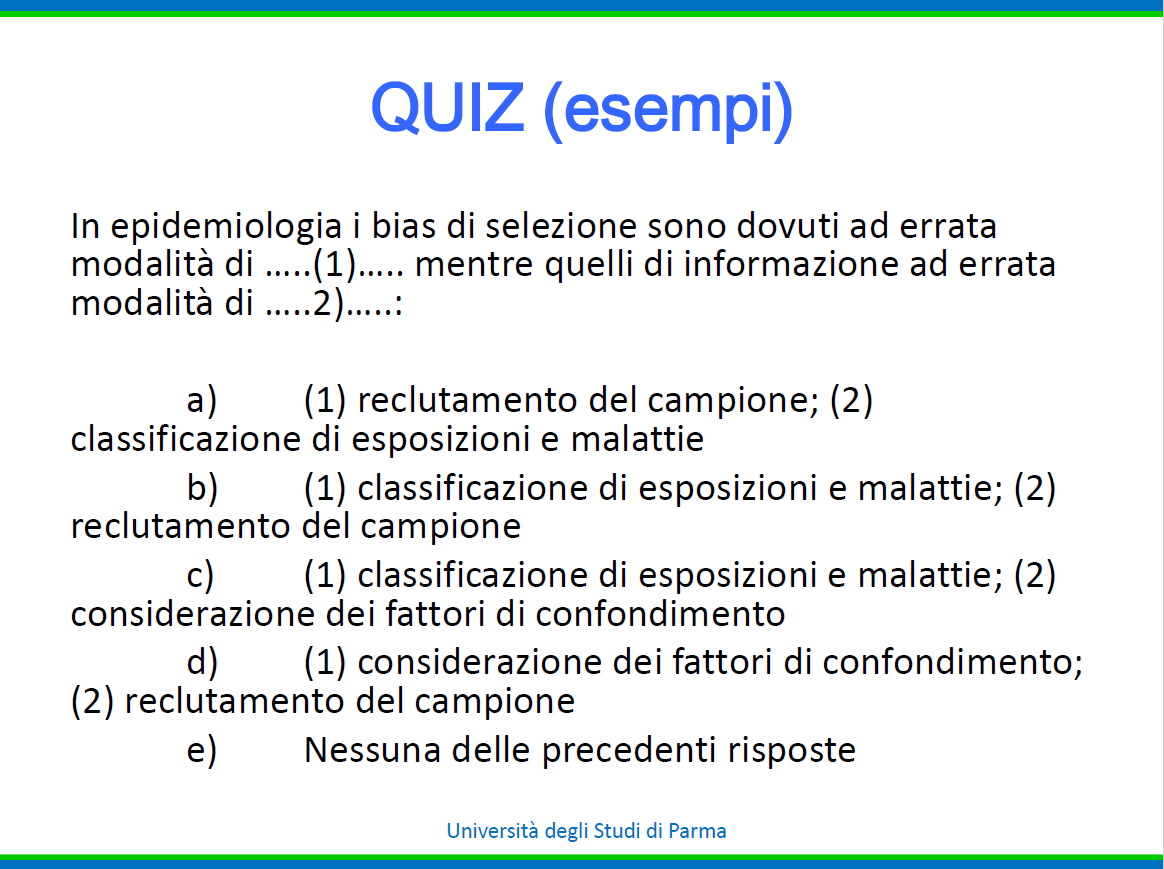
\includegraphics[width=0.7\textwidth]{05/image18.png}
\end{figure}

Risposta esatta: A.

